\documentclass[border=10pt]{standalone}
\usepackage{pgfplots}
\pgfplotsset{compat=1.18}
\usepgfplotslibrary{colormaps}

\begin{document}
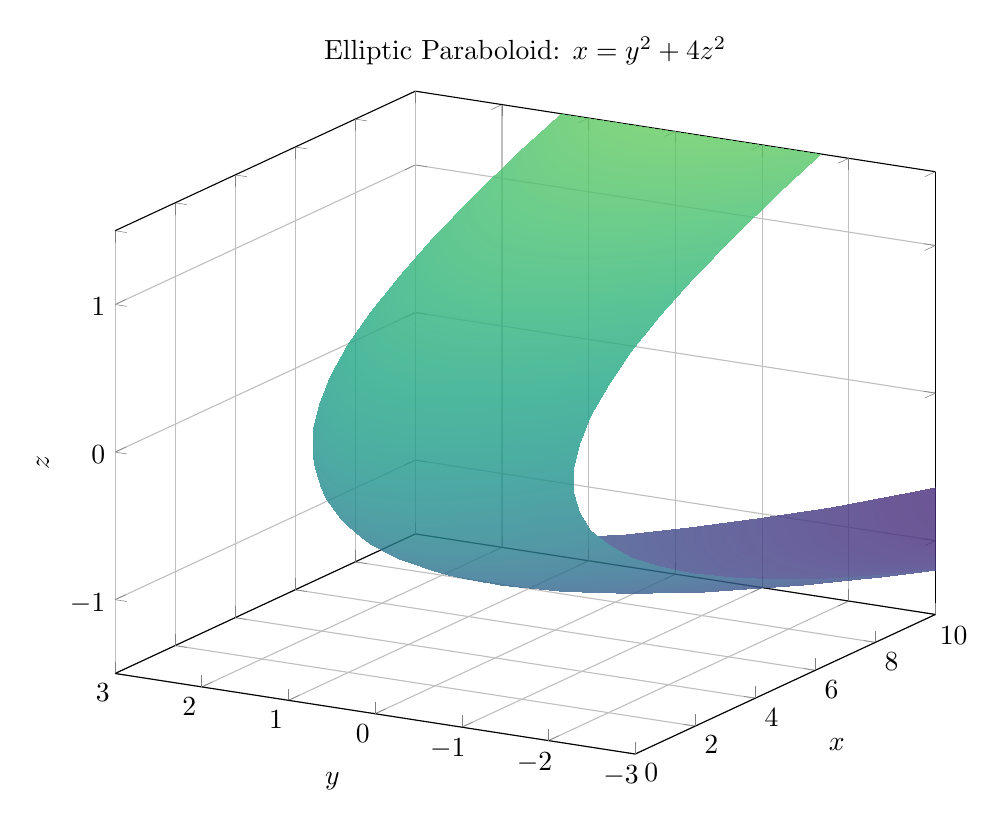
\begin{tikzpicture}
\begin{axis}[
    width=12cm,
    height=10cm,
    xlabel={$x$},
    ylabel={$y$},
    zlabel={$z$},
    title={Elliptic Paraboloid: $x = y^2 + 4z^2$},
    view={-60}{20},
    colormap/viridis,
    grid=major,
    zmin=-1.5,
    zmax=1.5,
    ymin=-3,
    ymax=3,
    xmin=0,
    xmax=10,
]
\addplot3[
    surf,
    domain=-3:3,
    y domain=-1.5:1.5,
    samples=40,
    samples y=30,
    shader=interp,
    opacity=0.8
] 
(y^2 + 4*x^2, y, x);
\end{axis}
\end{tikzpicture}
\end{document}